\documentclass[a4paper,10pt]{report}

% Language
\usepackage[UKenglish]{babel}    % define culture for rendering (eg., hyphenation rules)
\usepackage[T1]{fontenc}       % use utf8 fonts
\usepackage[utf8]{inputenc}      % input encoding is utf8
\usepackage{lmodern}             % use font Latin Modern

% Supreme boilerplating
\usepackage{etex}                % LaTeX 2.0 features on relics
\usepackage{microtype}           % Extremely anal typographic mode
\usepackage{url}                 % Ability to create URLs
\usepackage[hidelinks]{hyperref} % Makes intradocument links, eg., contents page
\usepackage{color}               % Adds colour features. Really.
\usepackage{graphicx}            % Adds image features

% Layout
\usepackage[a4paper]{geometry}   % In case I want to set margins etc.
\usepackage{setspace}            % For setting line spacing
\usepackage{enumerate}           % Allows different types of numbering
\onehalfspacing

% Actual Packages
\usepackage{fixme}
\usepackage[authoryear, round, sort]{natbib} % References
\usepackage{amsmath}             % Imports for maths things
\usepackage{amssymb}
\usepackage{amsthm}
\usepackage{empheq}              % For highlighting mathematics
\usepackage{tikz}
\usetikzlibrary{arrows,shapes,decorations.pathreplacing,decorations.pathmorphing,calc,patterns,scopes,trees,positioning,fit}
\usepackage{pgfplots}
\pgfplotsset{compat=1.7}
\pgfkeys{/pgf/number format/relative round mode=fixed}

% Bug Fixes
\usepackage{fixltx2e}            % LaTeX bugfixes (yes really)
% "fix the natbib spacing character" - Kevin Naud�
\makeatletter
\ifdefined \NAT@spacechar
	\def\NAT@spacechar{~}
\fi
\makeatother

\hypersetup{pageanchor=false}    % Wait until actual start of writing before making page anchors


%%%%%%%%%%%%%%%%%%%%%%%%%%%%%%%%%%%%%%%%%%%%%%%%%%%%%555
% Macros

% Restarts numbering and sets format to 1, 2, 3...
\newcommand \startrealnumbers { 
	\pagenumbering{arabic}
	\setcounter{page}{1} 
	\hypersetup{pageanchor=true}
}

% Renders a bibliography on its own page, and adds a contents reference.
\def \bibliographysection {
	\cleardoublepage
	\phantomsection
	\addcontentsline{toc}{chapter}{Bibliography}
	\bibliographystyle{authordate3}
	\bibliography{bibliography}
}

\newcommand \todo \fxwarning

\begin{document}

\title{A JIT-less, Register-Mapped, Statically-Typed Virtual Machine for Interpreters}
\author{Matthew Sainsbury}
\date{\today}

% Cover Page
\begin{titlepage}

		\maketitle
	
\end{titlepage}

\pagenumbering{roman}

% Prefaces
\nakedchapter{Acknowledgements}
	To all my loyal fans

\nakedchapter{Abstract}
	\todo{align this with project proposal}
	Traditional JIT-less high-level register virtual machines simulate virtual registers in random access memory (RAM) and load virtual registers from RAM whenever they are accessed \citep{caseregistervm}. This treatise investigates an alternative approach where virtual registers are mapped to physical registers, and instructions are dispatched not only on the opcode, but also on the operands of the instruction. To emulate a virtual instruction, the interpreter jumps to the appropriate code segment in a table of implementation code based on the instruction word to be executed. This table grows in a polynomial fashion with increased virtual registers, and therefore the performance balance between table size and register pressure is investigated.

\nakedchapter{Declaration of Own Work}


\tableofcontents

\nakedchapter{Glossary}
\begin{description}
	\item[Bytecode] Program code executed by a virtual machine.
	\item[Virtual Machine] A class of programs which translate code written for one architecture to another.
\end{description}


% Main document body
\chapter{Introduction}
	\startrealnumbers
	This treatise investigates a new implementation technique for interpreted virtual machines. Two ideas are presented: register mapping between virtual machine registers and real registers, and a new dispatch method which operates on full instruction words. It is thought \todo{Weazel words?} that these two novelties might allow a modern pipelined CPU to better predict the behaviour of the virtual machine by reducing the amount of data dependance.
	
	This section aims to establish the landscape of modern processor design and the problems which arise in virtual machine implementations, as well as describe the scope of this project.
	
	\section{Background}
		A virtual machine is a program that executes a machine code program by translating the instructions from one machine architecture to another. This allows a programmer to execute a program written for one architecture on a different architecture.
		
		A subclass of virtual machines---high-level virtual machines---are of interest in this project. A high level virtual machine runs programs for a machine which is imagined by its designer. This machine is typically more sophisticated and generic than real machines. As a consequence, a high-level virtual machine is an abstraction layer which hides the intricacies of any particular real machine. This virtual machine can be implemented for any physical architecture, resulting in the extremely useful property that code written for a virtual machine is very portable. The ``machine code'' that a high-level virtual machine executes is called its \emph{bytecode}. 
		
		The primary use for high-level virtual machines is in high-level interpreted languages, such as C$^\sharp$, Java and Python. High-level language interpreters are typically implemented with a compiler that compiles the input source code into an intermediary bytecode, which is then interpreted on a high level virtual machine. This technique is much faster than interpreting the source code line-by-line. Because the virtual machine is designed to support high-level features of interpreted languages, it is easier to write a compiler for the language targeting the virtual machine. This approach also helps to modularise the structure of the interpreter by seperating the language and context analysis structures from the host-specific implementation details \citep{structureinterpreters}.
		
		The interpretation of bytecode on any virtual machine is significantly slower than executing native code \citep{optimizingindirectbranch}. Just-in-time (JIT) compilation tries to bring ``the best of both worlds'' together. Modern JIT interpreters begin with the normal interpretation process, but while interpreting, profiles the executing bytecode to determine which parts of the bytecode would most benefit from native execution. Once it has identified these sections of bytecode, it compiles them into the host machine's instruction set and executes them natively instead of interpreting them \citep{historyjit}. Most popular virtual machines utilise JIT compilation, such as Java's JVM, and C$^\sharp$'s Common Language Runtime (CLR).
		
		Although JIT compilation is a good strategy to improve the performance of virtual machines, they have disadvantages in certain use cases. For instance, in multi-instance programs, where a program is started many times to produce many processes running the same code simultaneously. A real-world example of such a program is a web server, which spawns several identical program threads to serve web clients asynchronously.
		
		As shown in Figure \ref{fig:nativeprogram}, operating system kernels automatically arrange native multi-instance programs to share a read-only code space between instances \citep{sharedcodepatent}. This does not happen with an interpreted program, because the code is loaded by the interpreter, and not by the kernel itself. With an interpreter utilising a JIT compiler, each process will be doing its own tracing and JIT compilation of the bytecode, essentially compiling the same code over and over (Figure \ref{fig:interpretedprogram}). JIT compilation is a hefty procedure, so multiple compilations of the same identical code is not acceptable. Overcoming this problem require processes to have a mechanism to discover other running processes that are using the same interpreter, and then negotiate a code-sharing scheme. Implementing such a system would be very difficult. With this in mind, it is useful to explore opportunities for improvement in JIT-less interpreters so that situations where JIT compilation is inappropriate are not neglected. 
		
		Unfortunately, multi-instance applications have become much more common as CPUs increase in core count, and stagnate in clock frequency. With this in mind, ``traditional'' high-level virtual machines will be considered.
		
		\begin{doublefig}
			\begin{halffig}
				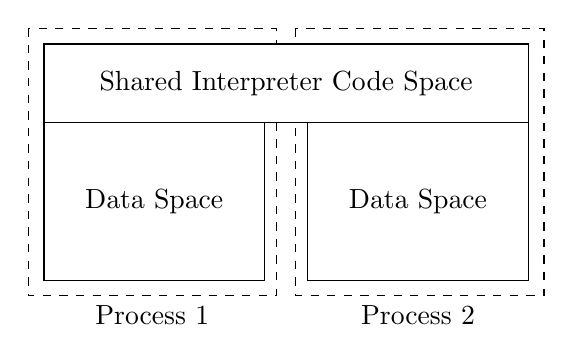
\begin{tikzpicture}
				\draw (-0.2, 0.2) [dashed] rectangle (2.95, -3.2) node[below] at (1.375, -3.2) {Process 1};
				\draw (3.2, 0.2) [dashed] rectangle (6.35, -3.2) node[below] at (4.75, -3.2) {Process 2};
				\draw (0,0) [fill=white] rectangle (6.15,-1) node[midway] {Shared Interpreter Code Space};
				\draw (0,-1) rectangle (2.8, -3) node[midway] {Data Space}; 
				\draw (3.35,-1) rectangle (6.15, -3) node[midway] {Data Space}; 
				\end{tikzpicture}
				\caption{Two native programs}
				\label{fig:nativeprogram}
			\end{halffig}
			\begin{halffig}
				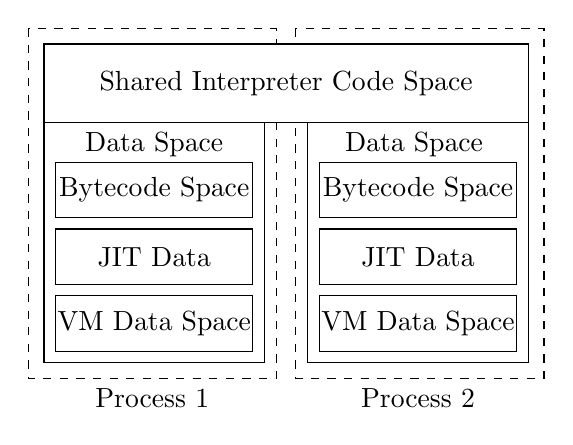
\begin{tikzpicture}
				\draw (-0.2, 0.2) [dashed] rectangle (2.95, -4.25) node[below] at (1.375, -4.25) {Process 1};
				\draw (3.2, 0.2) [dashed] rectangle (6.35, -4.25) node[below] at (4.75, -4.25) {Process 2};
				\draw (0,0) [fill=white] rectangle (6.15,-1) node[midway] {Shared Interpreter Code Space};
				\draw (0,-1) rectangle (2.8, -4.05) node[below] at (1.4,-1) {Data Space}; 
				\draw (3.35, -1) rectangle (6.15, -4.05) node[below] at (4.7,-1) {Data Space};
				\draw (0.15, -1.5) rectangle (2.65, -2.2) node[midway] {Bytecode Space};
				\draw (3.5, -1.5) rectangle (6, -2.2) node[midway] {Bytecode Space};
				\draw (0.15, -2.35) rectangle (2.65, -3.05) node[midway] {JIT Data};
				\draw (3.5, -2.35) rectangle (6, -3.05) node[midway] {JIT Data};
				\draw (0.15, -3.2) rectangle (2.65, -3.9) node[midway] {VM Data Space};
				\draw (3.5, -3.2) rectangle (6, -3.9) node[midway] {VM Data Space};
				\end{tikzpicture}
				\caption{Two interpreted programs}
				\label{fig:interpretedprogram}
			\end{halffig}
		\end{doublefig}
		
		\subsection{Traditional Virtual Machines}
			There are two general types of high-level virtual machine architectures: stack machines and register machines. 
			
			Unsurprisingly, a stack machine maintains a stack data structure where temporary values are stored, and the machine's instruction set consists mostly of operations on the stack. Figure \ref{fig:stackprogram} shows an example of code written for a stack machine. Notice that the operands of the instructions are implicit, and so instructions for stack machines tend to be shorter. This is the major difference between instructions for stack machines and register machines. 
		
			The bytecode of a stack machine is very simple. For each operation, a unique code (called an \emph{opcode}) is assigned. For instance, a word value~(``instruction word'') of \texttt{0x01} might represent push, while \texttt{0x02} might represent add, and so on. The introduction of literals, such as the $14$ and $8$ in the first two lines---as well as other types of additional data attached to instructions---complicates this picture, but the idea remains unchanged.
		
			A register machine contains a number of high-speed memory ``boxes'' into which temporary values are stored, called registers. Instructions generally specify which registers are involved in the operation~(``operands''). Figure \ref{fig:registerprogram} shows the same program for a register machine. In the \texttt{add} instruction, the value of \texttt{regA} is added to \texttt{regB}, and the result is stored in \texttt{regA}. This is a convention in assembly programming which will be used throughout the text.
		
			A register machine's bytecode is different, because the operands of the instruction need to be part of the instruction encoding. Typically this is implemented using bitfields. For example, consider a twelve-bit instruction word. We can reserve the first 4 bits for the opcode. This gives us a maximum of 16 opcodes. The next four bits of the instruction word can encode the first operand as an enumeration, and the same for the last four bits which can encode the second operand. If an instruction only has one operand, the last four bits are undefined. This is illustrated in Figure \ref{fig:bitfields}
			
			\begin{myfigure}
					\texttt{
						\begin{tabular}{ | l | r | r |r | }
							\hline
							Meaning & opcode & dest & src \\ 
							\hline
							add regA, regB  & 0001 & 0000 & 0001 \\
							\hline
							add regD, regC & 0001 & 0011 & 0010 \\
							\hline
							divide regB, regA & 0010 & 0001 & 0000 \\
							\hline
							print regA & 0011 & 0000 & 0000 \\
							\hline
						\end{tabular}
					}
					\caption{Register instructions using bitfields}
					\label{fig:bitfields}
			\end{myfigure}
			
			\begin{doublefig}
				\begin{halffig}
					\begin{lstlisting}
push 14
push 8
add
push 7
divide
print
					\end{lstlisting}
					\caption{Stack machine program}
					\label{fig:stackprogram}
				\end{halffig}
				\begin{halffig}
					\begin{lstlisting}
mov regA, 14
mov reg1, 8
add regA, regB
mov regB, 7
divide regA, regB
print regA
					\end{lstlisting}
					\caption{Register machine program}
					\label{fig:registerprogram}
				\end{halffig}
			\end{doublefig}
			
			\todo{Should I talk about dispatching, and virtual machine implementation in general?}
			
		\subsection{The Nature of Modern Processors}
			The landscape of processor design has changed significantly in the last thirty years. Rather than producing performance gains by arbitrarily increasing processor clock speeds, modern processor designers rely on trying to increase the per-cycle efficiency of their processors, using techniques such as instruction-level parallelism, larger and more complex cache systems, and speculative optimisation. These design issues caught the interest of academics and engineers in the 1980's \citep{modernprocessordesign}. Some of these topics will be briefly discussed in this section.
			
			\subsubsection{Instruction-Level Parallelism}
			Traditional processors executed machine instructions one at a time. Every clock cycle, an instruction would be fetched, decoded, and executed. The result of this method is that activity on a processor would move through the architecture componentwise. Only one part of the process would be ``working'' at any time---for instance, when an instruction was being decoded, the entire execution component of the processor was unused.
			
			On a processor with instruction-level parallelism, these functions can operate in parallel. An instruction can be fetched while another instruction is being decoded, and yet another instruction's operands are being fetched. A processor that can operate this way is said to have an \emph{instruction pipeline.} This results in far better utilisation of processor hardware, but introduces complexity in the processor. For instance, if one instruction writes to a memory address, and later instruction reads from the same address, the second instruction cannot complete the operand fetch stage until the first instruction has been executed. A situation where an instruction has to wait for another to complete is known as a \emph{pipeline stall,} and is a subject of much academic writing and engineering effort.
			
			\subsubsection{Cache Arrangement}
			Modern processors contain portions of high-speed memory which act as a cache to the main memory of the machine. The behaviour of this cache is an important factor for processor performance, because main memory is quite slow compared to the speed of a CPU. Modern caches are orders of magnitude larger than processors twenty years ago. 
			
			Most modern processors contain a series of specialised caches. For instance, a fourth-generation Intel Core processor has three grades or \emph{levels} of cache, and make a distinction between cache for instructions and cache for program data. Figure \ref{fig:cachenumbers} shows the arrangement of cache on such a processor. As can be seen, L1 cache is much faster, but much smaller than L2 cache. The latency in L1 instruction cache is not shown because instruction fetch is transparent to programs, but it does influence branch prediction (see later). It is advantageous for a program if most of its application data can fit in L1 data cache, and most of its code can fit in L1 instruction cache. 
			
			\begin{myfigure}
				\begin{tabular}{ | l | l | l | l | }
					\hline
					Level & Type & Size & Latency \\ 
					\hline
					\multirow{2}{*}{L1} & Instruction & 32KB & N/A \\
					& Data & 32KB & 4 cycles \\
					\hline
					L2 & Data & 256KB & 11 cycles \\
					\hline
					L3 & Data & Varies & Varies \\
					\hline
				\end{tabular}
				\caption{Cache on 4th-Gen Intel Core CPUs \citep{optimisationreference}}
				\label{fig:cachenumbers}
			\end{myfigure}
			
			\subsubsection{Branch Prediction \& Branch Target Prediction}
			Branch prediction in a process refers to the processor's ability to continue the pipelining process during a branch instruction. Ordinarily, the location of the next instruction is known to the processor---it is simply the instruction adjacent to the previous one. If the previous instruction was an instruction to branch (go somewhere else in the program), the picture becomes more complex. There are three types of branches worth mentioning:
			
			\begin{description}
				\item[Unconditional Branch:] This instruction always causes the processor to jump to the same location. The target of the branch is known as soon as the instruction is decoded.
				\item[Conditional Branch:] This branch type branches to a constant location if a condition is true. For instance, if a register is zero (``branch if zero''). The location of the next instruction is only known once the branch instruction is executed.
				\item[Indirect Branch:] A branch whose branch location is based on program data, whether in memory or in a register, or both. 
			\end{description}
			
			An unconditional branch is the easiest branch to pipeline, since the location of the next instruction is encoded in the branch instruction itself. The next instruction can be fetched as soon as the branch instruction is decoded. 
			
			A conditional branch is harder to pipeline because it is not known whether the condition is true or false before the instruction is executed, and thus what the next instruction should be. To prevent pipeline stalls on conditional branch instructions, modern processors implement a \emph{branch predictor}. The branch predictor will use some heuristic to predict the conditional, and load the most likely next instruction. A pipeline stall will only occur if the prediction was wrong---this delay is known as the \emph{misprediction penalty}.
			
			An indirect branch is the worst type of branch for a pipelined processor. It is very hard to predict because the branch location could depend on any data anywhere in main memory or in registers. This influence that data has on the behaviour of the program is known as \emph{data dependance} and is to be avoided whenever possible. Modern processors implement a \emph{branch target predictor} in an attempt to reduce the number of pipeline stalls. A branch target predictor is not to be confused with a branch predictor---a branch predictor predicts whether the branch will be taken, whereas a branch target predictor tries to predict where the branch will lead. A conditional branch can only lead two places---the next instruction, or the constant branch location.
			
			One common branch target predictor is a \emph{branch target buffer} (BTB). A branch target buffer maintains a table storing the last target location of each indirect branch encountered. Thus a BTB makes the assumption that an indirect branch target is unlikely to change  \citep{yeti}. This strategy works well if an indirect branch always branches to the same location, but is no help if it is always different.
			
			These concepts form the background to this research, and the problems which motivate it.
	
	\section{Problem Description}
		Most physical machines are register machines. It is thought that the use of real machine registers to store the values of the virtual machine registers will help to make the operation of virtual machine programs more transparent to the physical CPU by reducing data-dependant fetches from main memory, where virtual machine registers are usually stored. Unfortunately, unlike virtual registers that are implemented in memory, real registers cannot be accessed by ``reference'' \citep{caseregistervm}. This difference complicates the implementation of a register-mapped virtual machine.
		
		Despite these difficulties, it is worthwhile to investigate designs of JIT-less register virtual machines that attempt to narrow the divide between the host and guest architecture.
	
		\todo{Do I need more?}
		
	\section{Purpose and Scope}
		The goal of this project is to investigate the feasibility of JIT-less register virtual machines for interpreters running on a modern architecture. To this end, a high-level register virtual machine will be implemented with some unique architecture features that have not been investigated or thought feasible previously.
		
		A novel dispatch process will be investigated that seeks to allow the use of physical machine registers in the implementation of virtual machine registers. To circumvent the problem of referencing real machine registers, the virtual machine will dispatch not only based on the opcode of each instruction, but on the instruction as a whole. In other words, an implementation will exist for every combination of operands in each virtual machine instruction.
	
		An instruction set architecture will be designed which will be tailored for such a dispatch method. It is anticipated that having implementations for every combination of operands in each virtual machine instruction will cause the virtual machine implementation to become very large, and so the design of the instruction set architecture will focus on keeping the number of unique instructions low.
		
		The virtual machine will target the Intel 64 host machine architecture.
		
		\subsection{Limitations}
			As the virtual machine implementation becomes very large, it will become unsuitable for operation on machines with small L1 and L2 instruction caches, because large portions of the virtual machine implementation will not remain in the instruction cache. The result is a virtual machine that is actually slower than traditional virtual machines. We will consider only modern processors with reasonably large first-level cache, for instance, the current Intel Core i7 range of processors containing 32KB of L1 instruction cache.
			
			Assuming any virtual machine register can be used as an operand for any instruction, the size of the virtual machine implementation proportional to:
			
			\[
				\sum_{o~\in~opcodes} r^n : 
					\begin{array}{l}
						n \coloneqq \text{number of operands for o} \\
						r \coloneqq \text{number of virtual machine registers}
					\end{array}
			\] 
			
			Every additional virtual machine register increases the size of the virtual machine by a polynomial factor. At some point, any performance gain received by exposing more physical registers will be negated by increasing incidence of cache misses. This is a source of a practical limitation on the number of registers in the virtual machine's architecture.
			
				
	\section{Overview of Treatise Structure}
		\todo{Will have to wait until the rest of the treatise exists for this! Tip: Design this for someone who doesn't feel like reading the whole thing. Make it easy to find specific, interesting sections.}

% 10-12 pages
\chapter{Problem Exposition}
	\section{Literature Review}
		\cite{structureinterpreters} reflect on why spending research and engineering effort on optimising interpreters is a worthwhile endeavour. Creating a machine abstraction layer between original source code and host machine architecture greatly simplifies the writing of compilers that target many platforms. Without such an abstraction layer for each host machine, a separate version of the compiler targeting that platform must be developed. Interpreters allow compilers to be more versatile with little effort. In a high-level language interpreter utilising a virtual machine, only the interpreter portion needs to be rewritten for different platforms, (or perhaps not even the interpreter if a high-level language is used to implement the interpreter) and the compiler remains the same. Interpreters tend to be simple compared to compilers targeting machine code, so this advantage is quite significant. Compared to native execution, interpreters also offer opportunity for more powerful usability features like debuggers, and have faster compilers, improving the write-compile-test cycle of modern software development methods.
		
		A good design of a high-level virtual machine is one that is both easy to compile code for (sophisticated) and allows for fast interpretation (low overhead).
		
		The feature that is present in all virtual machine interpreters is a dispatch process. Dispatch refers to the process of fetching, decoding, and starting the execution of a virtual machine instruction. Dispatch technique can have the biggest effect on the performance of a virtual machine.
		
		The most efficient dispatch is direct threaded code. ``Threading'' in this case does not refer to ``multithreading'', but instead to a much older type of code structuring technique. In this method, a virtual machine instruction is actually the address of the code that implements that instruction. This is illustrated in Figure \ref{fig:directthreading}. Notice the line `\texttt{jmp *pc++}'. This is an indirect branch. An indirect branch is an inescapable consequence of the dispatch process. Direct threading is efficient because, although it contains an indirect branch, there is little other overhead.
		
		\begin{myfigure}
				\begin{lstlisting}
start:
  pc = bytecode
  jmp *pc++

bytecode:
  &add
  &divide
  &print

add:
  //implementation
  jmp *pc++

divide:
  //implementation
  jmp *pc++

print:
  //implementation
  jmp *pc++

				\end{lstlisting}
				\caption{Direct Threading Dispatch}
				\label{fig:directthreading}
		\end{myfigure}
		
		The reason that the jump instruction occurs at the end of each implementation is that duplicating the indirect jump increases the utilisation of a branch target prediction, since there is an entry in the branch target buffer for each indirect branch instruction. If there was one common jump instruction, the BTB would always predict that the next instruction is the same as the previous one, which is not usually the case. This will be better explained further in this chapter.
		
		Other techniques for improving the accuracy of branch target prediction have been investigated, and some more interesting ones are summarized by \cite{optimizingindirectbranch}. 
		
		One interesting finding of that paper was that branch prediction in loops could be improved if no duplicate instructions occur in the loop. Branch prediction accuracy can be 100\% in that case, because the next instruction can always be predicted based only on the current instruction. \citeauthor{optimizingindirectbranch} suggested a counterintuitive technique of duplicating instructions to allow compilers to ensure that each instruction is only used once in a loop.
		
		Another interesting technique investigated by \citeauthor{optimizingindirectbranch} is the use of `superinstructions' which are groups of instructions with a single opcode. By combining instructions into more complex instructions which are used less often, this technique can reduce branch prediction failures.
		
		Traditionally, the high level virtual machines implemented in interpreters are stack machines. Stack machines are used over register machines for a few reasons. Instructions for stack machines are smaller, because instruction operands are implicit. This means that instruction fetching is faster. It is easier to compile code for a stack machine than a register machine because the compiler does not need to implement a register allocator \citep{caseregistervm}. However, \cite{stackregistershowdown} found that an efficient register virtual machine can execute benchmarks 32\% faster than an analogous stack machine. 
		
		\cite{caseregistervm} mentions that the first successful virtual machine interpreter ran stack-based P-code for Pascal. This was the first in a large family of stack-based bytecodes for popular languages like Smalltalk, Java and the Common Intermediate Language (CIL). This suggests that there might be historic factors involved in the prevalence of stack based virtual machines.
		
		\cite{fastjava} believes that interpreters are not well designed to suit modern architectures features like pipelining, branch prediction and caches. They also provide encouragement by saying, ``if interpreters can be made much faster, they will become suitable for a wide range of applications that currently need a JIT.''
		
		\subsection{Relevant Previous Work}
		The practice of mapping virtual machine resources to host machine registers has been investigated for stack machines by \cite{stackcaching}. Ertl measured the performance of stack machines which kept the top few elements of the stack in registers. He found that direct mapping of stack positions to machine registers was only useful for the case where just the top element of the stack was cached in a register. Further caching resulted in too many load-store instructions to shuffle register values around when positions on the stack change.
		
		Ertl also attempted a technique he calls ``dynamic stack caching'' where stack elements are cached in whatever register is convenient, and an internal state machine remembers the mapping between stack context and registers. The technique employs multiple versions of code to emulate each virtual machine instruction; the version which is executed depends on the current state of the state machine (register-stack state mapping). Ertl found that this technique halves the cost of operand fetching for each additional register involved in the caching, but adds an instruction dispatch cost because of the increased number of states. A possible explanation for this is the increase in dispatch complexity, and increased cache miss rate due to the large number of states.
		
		In the same paper, Ertl writes the first mention of the idea of achieving register mapping between a register virtual machine and a host register machine through a table of implementations for each combination of opcode and operands. However, the idea is quickly dismissed, as it would ``cause code explosion, and will probably suffer a severe performance hit on machines with small first-level caches.'' The R4000 MIPS processor was a contemporary example, having only 8 KB of level one (L1) instruction cache.
	
		The state of cache availability has changed for modern processors. Consequently, this approach deserves further investigation. Modern processors have significantly larger cache sizes. For example, 4th generation Intel Core processors have 32 KB of L1 instruction cache \citep{optimisationreference}, four times as much as the R4000. They also have much larger second and third level caches.
		
		\todo{Should I spend much more effort on this subsection?}
	
		
	\section{Difficulties}
		Interpreters spend most of their execution time on instruction dispatch \citep{modernarchvm}. The main contributor is usually an indirect branch to the implementation code for the currently executing virtual machine instruction \citep{optimizingindirectbranch}. Every interpreter has at least one indirect branch in dispatch code \citep{modernarchvm}. Because these indirect branches are in the instruction dispatch portion of the interpreter, they are executed for every virtual machine instruction. This closely couples interpreter speed to efficiency of branching.
		
		Modern architectures tend to have long pipelines and perform branch target prediction to load the target of an upcoming branch before the branch instruction is executed. Branch target misprediction is very expensive in these architectures, because the execution of a branch happens late in the pipeline but affects the start of the pipeline \citep{optimizingindirectbranch}.
				
		Traditional interpreter designs that were optimal on older architectures perform poorly on modern pipelined architectures because branch prediction accuracy is a big factor on performance on these architectures. These interpreter designs hide the logic governing branching patterns from the branch predictor. All the host processor sees is branches that depend on data, and is not aware that this data stream represents a program. The machine abstraction layer causes the virtual machine to inherit the weaknesses of deep pipelining from the modern host processor, while abstracting away opportunities of dynamic optimisation in the modern host.
		
		\cite{yeti} explains this by saying ``the control transfer from one body to the next is data dependent on the sequence of instructions making up the virtual program.'' This is an atypical scenario for modern processors, and they are not designed optimally for this task.
		
		Consider the virtual machine dispatch process on a modern processor with a branch target buffer (BTB). When a dispatch's indirect branch is encountered for the second time, BTB predicts the target will remain the same. However, this is not the case for the dispatch's branch, because the indirect branch is based on the current virtual machine opcode, which could be any of the instructions in the virtual machine instruction set. For each of these opcodes, the interpreter will branch to a particular section of code to emulate the virtual machine instruction. In other words, \emph{the BTB prediction will be accurate only if the opcode being dispatched is the same as the previous dispatch}. Because it is not very likely that the virtual machine will see many of the same opcode over and over, the BTB fails to predict the branch target most of the time. Opcodes ``fight'' for the single target record in the BTB that corresponds with the indirect branch in the dispatch code. It is now clear why the illustration of a conventional interpreter in Figure \ref{fig:directthreading} duplicates the indirect branch per instruction.
		
		\begin{myfigure}
			\begin{tabular}{c c}
				{
				\begin{lstlisting}
start:
  pc = bytecode
  jmp *pc++

bytecode:
  &add
  &add
  &divide
  &add
  &print

add:
  //implementation
  jmp *pc++

divide:
  //implementation
  jmp *pc++

print:
  //implementation
  jmp *pc++
				\end{lstlisting}
			} & 
			{
				\begin{tikzpicture}
					\draw (0,7) -- (1, 7);
				\end{tikzpicture}
			}
			\end{tabular}
			\caption{Illustration of Indirect Branch Problems in Interpreters}
			\label{fig:interpreterbtb}
			\todo{Can't figure out drawing arrows on code}
		\end{myfigure}
		
		\cite{structureinterpreters} found that the branch misprediction penalty consumes up to half of the execution time on some interpreters. This high proportion is a result of the fact that most of an interpreter's time is spent in the instruction dispatch process.
		
		One way to get around this problem is by duplicating the indirect branch instruction, resulting in a separate BTB entry for each branch instruction \citep{fastjava}. This can be done by duplicating the dispatch code at the end of each virtual instruction implementation, instead of jumping back to a common dispatch code. In contrast, the traditional focus in branch optimisation was to make the code path as short as possible.
		
% 10-12 pages
\chapter{Solution Design}
	In this section the design of the virtual machine will be discussed. \todo{more}
	
	The overarching design goal for this virtual machine is to enable register mapping between virtual machine and host machine.
	
	In traditional virtual machines, an implementation for a virtual machine instruction will look like Figure \ref{fig:operandfetch}. Notice how the virtual registers are implemented as an array in memory, and that the index of the virtual register is encoded into the instruction word (a bitfield, as explained earlier). If we are to store the virtual registers in real registers, we cannot access the register using an index.
	
	\begin{myfigure}
		\begin{lstlisting}
add(instr):
  ai = getSourceRegisterIndex(instr) //decode
  bi = getDestinationRegisterIndex(instr) //decode
  a = registers[ai]
  b = registers[bi]
  registers[bi] = a+b
  dispatch()
		\end{lstlisting}
		\caption{Operand Load/Store in Conventional Implementations}
		\label{fig:operandfetch}
	\end{myfigure}
	
	Instead, we will duplicate the implementation code for every combination of registers, as in Figure \ref{fig:dupimplementation}. Notice how the implementation is much simpler (we have managed to remove all the operand fetch code from before), although there is a significantly larger amount of code. By hard-coding the registers instead of dynamically accessing them, we are able to circumvent the indexing issue.
	
		\begin{myfigure}
			\begin{lstlisting}
			add_0_0:
			regA = regA + regA
			dispatch()
			add_0_1:
			regA = regA + regB
			dispatch()
			add_0_2:
			regA = regA + regC
			dispatch()
			...
			add_1_0:
			regB = regB + regA
			dispatch()
			add_1_1:
			regB = regB + regB
			dispatch()
			...
			
			\end{lstlisting}
			\caption{Operand Load/Store in Conventional Implementations}
			\label{fig:dupimplementation}
		\end{myfigure}
	
	This method raises the problem that the virtual machine implementation code might become extremely large. If this happens, it is less likely to be cached by the processor and will perform badly. We repeat the equation presented in the limitations discussion which characterizes the size of the implementation:
	
	\[
	\sum_{o~\in~opcodes} r^n : 
	\begin{array}{l}
	n \coloneqq \text{number of operands for o} \\
	r \coloneqq \text{number of virtual machine registers}
	\end{array}
	\] 
	
	There are several things we can do to attempt to reduce the inevitably large size of the implementation. The most obvious thing we can do is reduce the number of instructions supported by the VM architecture. This is more possible in high-level virtual machines than real machines, because the instructions tend to be more sophisticated. The second thing we can do is to reduce the number of registers exposed through the VM architecture. Because the size of the implementation has a polynomial relation to the number of exposed registers, this will probably have the largest effect. Our last attempt to reduce the size of the implementation will be to prohibit certain trivial combinations of operands for certain instructions. For instance, the instruction `\texttt{sub regA, regA}' is useless because the result will always be the same as `\texttt{mov regA, 0}'. Similar arguments lead us to remove combinations like `\texttt{xor regA, regA}', `\texttt{and regA, regA}' and so on. Removing these instructions from our specification means we can remove their implementations, because every combination of operands has its own implementation in our virtual machine.
	
	Since our virtual machine is designed to be run as a user process under an operating system, we should include instructions that help the program interact with its environment under the operating system. We call these instructions ``pragmatic'' instructions.
	
	With all these constraints and goals in mind, we can design the virtual machine architecture.
	
	\section{Virtual Machine Architecture Design}
		When designing the virtual machine architecture, it will be beneficial to remember this succinct heuristic by \cite{structureinterpreters}: ``Well-designed VMs are tailored for both easy compilation from the source language and fast interpretation on real machines.'' \todo{too fluffy?}
		
		Our virtual machine will be developed for a static language. Consequently, we do not have to do type checking in the virtual machine. Registers in our virtual machine will notionally be one of two types---64-bit integer or pointer. The machine will have six general purpose registers, each of which can contain either a pointer or an integer. However, it is illegal to treat a pointer as an integer or vice versa. For this reason, a general-purpose register $g_i$ can be thought of as two distinct registers: an integer $r_i$ and a pointer $p_i$, only one of which is ``alive'' at any time. In fact, on real architectures that make a distinction between pointers an integers, these two ``virtual registers'' will be mapped to two distinct physical registers, so our strange convention is justified.
		
		Because this is a high-level virtual machine, pointers work like high-level languages in which pointer arithmetic is transparent. It is illegal to do arithmetic on pointers. This decision was made to make the interpreted language memory safe.
		
		There are two notional registers which are not visible to the programmer at all. These are \texttt{pc}, the virtual machine instruction pointer, and \texttt{fp} the stack frame pointer.
		
		Instructions are sixteen bits long. Unlike the majority of virtual machines, the instruction words are not bitfields. Since every unique instruction word corresponds to its own implementation code, and dispatch occurs over the entire word, bitfields serve no purpose, and actually make token threading more difficult because instructions with bitfields are not sequential.
		
		An instruction is sometimes followed by a sixteen-bit immediate value. This immediate can be either a sixteen-bit constant, or a relative displacement to a position elsewhere in the program. This interpretation depends on the preceeding instruction semantics.
		
		A pointer can refer to one of three data structures: an object, an array of integers, or an array of pointers. An object is defined in a prototype which has the format specified in Figure \ref{fig:objproto}.
		
		\begin{myfigure}
			\begin{tabular}{|l|l| }
				\hline
				Word & Meaning \\
				\hline
				0 & Number of fields ($n$) \\
				\hline
				$i \in 1, 2, ...$ & Bitmap: bit $b$ is set if field $i\times64 + b$ is a pointer \\
				\hline
			\end{tabular}
			\caption{Object Prototype Definition}
			\label{fig:objproto}
		\end{myfigure}
			
		We now present our instruction set.
		\todo{Notational Conventions}
		\todo{Omg a lot of the PC-relative are wrong here}
		\subsection{Arithmetic Operations}
		
		\begin{longtable}{|p{10em}|p{30em}|}
			\hline
			\multirow{2}{*}{Instruction} & Meaning \\
			& $RTL~Description$ \\
			\hline
			\texttt{add $r_i$, $r_j$} & Add an int in register $r_j$ to $r_i$ \\
			& $\begin{array}{lcl} 
			r_i \leftarrow (r_i + r_j)_{64} \\
			pc \leftarrow pc + 2  
			\end{array}$ \\
			\hline 
			\texttt{addc $r_i$, $const_{64}$} & Add a constant int to $r_i$ \\
			& $\begin{array}{lcl} 
			r_i \leftarrow (r_i + const)_{64} \\
			pc \leftarrow pc + 4  
			\end{array}$ \\
			\hline 
			\texttt{sub $r_i$, $r_j$} & Subtract $r_j$ from $r_i$, $i\neq j$ \\
			& $\begin{array}{lcl} 
			r_i \leftarrow (r_i - r_j)_{64} \\
			pc \leftarrow pc + 2  
			\end{array}$ \\
			\hline 
			\texttt{csub $const_{64}$, $r_i$} & Subtract constant from $r_i$ \\
			& $\begin{array}{lcl} 
			r_i \leftarrow (const - r_i)_{64} \\
			pc \leftarrow pc + 4
			\end{array}$ \\
			\hline 
			\texttt{mul $r_i$, $r_j$} & Multiply $r_i$ by $r_j$ \\
			& $\begin{array}{lcl} 
			r_i \leftarrow (r_i \times r_j)_{64} \\
			pc \leftarrow pc + 2
			\end{array}$ \\
			\hline 
			\texttt{mulc $r_i$, $const_{64}$} & Multiply $r_i$ by constant \\
			& $\begin{array}{lcl} 
			r_i \leftarrow (r_i \times const)_{64} \\
			pc \leftarrow pc + 4
			\end{array}$ \\
			\hline 
			\texttt{div $r_i$, $r_j$} & Divide $r_i$ by $r_j$, $i \neq j$. Store remainder in $r_0$ \\
			& $\begin{array}{lcl}
			div \leftarrow (r_i \div r_j)_{64} \\
			r_0 \leftarrow (r_i ~\%~ r_j)_{64} \\
			r_i \leftarrow div \\
			pc \rightarrow pc + 2
			\end{array}$ \\
			\hline 
			\texttt{divc $r_i$, $const_{64}$} & Divide $r_i$ by constant. Store remainder in $r_0$ \\
			& $\begin{array}{lcl}
			div \leftarrow (r_i \div const)_{64} \\
			r_0 \leftarrow (r_i ~\%~ const)_{64} \\
			r_i \leftarrow div \\
			pc \rightarrow pc + 4
			\end{array}$ \\
			\hline 
			\texttt{cdiv $const_{64}$, $r_i$} & Divide constant by $r_i$. Store result in $r_i$. Store remainder in $r_0$ \\
			& $\begin{array}{lcl}
			div \leftarrow (const \div r_i)_{64} \\
			r_0 \leftarrow (const ~\%~ r_i)_{64} \\
			r_i \leftarrow div \\
			pc \rightarrow pc + 4
			\end{array}$ \\
			\hline
		\end{longtable}
		
		\subsection{Bit Manipulation}
		\begin{longtable}{|p{10em}|p{30em}|}
			\hline \endfoot
			\hline 
			\multirow{2}{*}{Instruction} & Meaning \\*
			& $RTL~Description$ \\
			\hline \endhead
			\texttt{and $r_i$, $r_j$} & Bitwise and $r_j$ to $r_i$, $i \neq j$ \\*
			& $\begin{array}{lcl}
			r_i \leftarrow (r_i ~\&~ r_j)_{64} \\
			pc \leftarrow pc + 2
			\end{array}$ \\
			\hline
			\texttt{andc $r_i$, $const_{64}$} & Bitwise and const to $r_i$ \\*
			& $\begin{array}{lcl}
			r_i \leftarrow (r_i ~\&~ const)_{64} \\
			pc \leftarrow pc + 4
			\end{array}$ \\
			\hline
			\texttt{or $r_i$, $r_j$} & Bitwise or $r_j$ to $r_i$, $i \neq j$ \\*
			& $\begin{array}{lcl}
			r_i \leftarrow (r_i ~|~ r_j)_{64} \\
			pc \leftarrow pc + 2
			\end{array}$ \\
			\hline
			\texttt{orc $r_i$, $const_{64}$} & Bitwise or $const$ to $r_i$ \\*
			& $\begin{array}{lcl}
			r_i \leftarrow (r_i ~\&~ const)_{64} \\
			pc \leftarrow pc + 4
			\end{array}$ \\
			\hline
			\texttt{xor $r_i$, $r_j$} & Bitwise xor $r_j$ to $r_i$, $i \neq j$ \\*
			& $\begin{array}{lcl}
			r_i \leftarrow (r_i \wedge{} r_j)_{64} \\
			pc \leftarrow pc + 2
			\end{array}$ \\
			\hline
			\texttt{shl $r_i$, $r_j$} & Logical shift left $r_i$ by $r_j$, $i \neq j$ \\*
			& $\begin{array}{lcl}
			r_i \leftarrow (r_i \ll (r_j ~\&~ 0xFF))_{64} \\
			pc \leftarrow pc + 2
			\end{array}$ \\
			\hline
			\texttt{shlc $r_i$, $const_{16}$} & Logical shift left $r_i$ by $const$ \\*
			& $\begin{array}{lcl}
			r_i \leftarrow (r_i \ll (const ~\&~ 0xFF))_{64} \\
			pc \leftarrow pc + 4
			\end{array}$ \\
			\hline
			\texttt{cshl $const_{64}$, $r_i$} & Logical shift left $const$ by $r_i$ \\*
			& $\begin{array}{lcl}
			r_i \leftarrow (const \ll (r_i ~\&~ 0xFF))_{64} \\
			pc \leftarrow pc + 4
			\end{array}$ \\
			\hline
			\texttt{shr $r_i$, $r_j$} & Logical shift right $r_i$ by $r_j$, $i \neq j$ \\*
			& $\begin{array}{lcl}
			r_i \leftarrow (r_i \gg (r_j ~\&~ 0xFF))_{64} \\
			pc \leftarrow pc + 2
			\end{array}$ \\
			\hline
			\texttt{shrc $r_i$, $const_{16}$} & Logical shift right $r_i$ by $const$ \\*
			& $\begin{array}{lcl}
			r_i \leftarrow (r_i \gg (const ~\&~ 0xFF))_{64} \\
			pc \leftarrow pc + 4
			\end{array}$ \\
			\hline
			\texttt{cshr $const_{64}$, $r_i$} & Logical shift right $const$ by $r_i$ \\*
			& $\begin{array}{lcl}
			r_i \leftarrow (const \gg (r_i ~\&~ 0xFF))_{64} \\
			pc \leftarrow pc + 4
			\end{array}$ \\
			\hline
			\texttt{sar $r_i$, $r_j$} & Arithmetic shift right $r_i$ by $r_j$, $i \neq j$ \\*
			& $\begin{array}{lcl}
			r_i \leftarrow (r_i \ggg (r_j ~\&~ 0xFF))_{64} \\
			pc \leftarrow pc + 2
			\end{array}$ \\
			\hline
			\texttt{sarc $r_i$, $const_{16}$} & Arithmetic shift right $r_i$ by $const$ \\*
			& $\begin{array}{lcl}
			r_i \leftarrow (r_i \ggg (const ~\&~ 0xFF))_{64} \\
			pc \leftarrow pc + 4
			\end{array}$ \\
			\hline
			\texttt{csar $const_{64}$, $r_i$} & Arithmetic shift right $const$ by $r_i$ \\*
			& $\begin{array}{lcl}
			r_i \leftarrow (const \ggg (r_i ~\&~ 0xFF))_{64} \\
			pc \leftarrow pc + 4
			\end{array}$ \\
		\end{longtable}
		
		\subsection{Data Movement}
		\begin{longtable}{|p{10em}|p{30em}|}
			\hline \endfoot
			\hline 
			\multirow{2}{*}{Instruction} & Meaning \\*
			& $RTL~Description$ \\
			\hline \endhead
			\texttt{mov $r_i$, $r_j$} & Move the value in $r_j$ to $r_i$, $i \neq j$ \\*
			& $\begin{array}{lcl}
			r_i \leftarrow r_j \\
			pc \leftarrow pc + 2
			\end{array}$ \\
			\hline
			\texttt{movp $r_i$, $r_j$} & Make $r_i$ point to the same object as $r_j$, $i \neq j$ \\*
			& $\begin{array}{lcl}
			r_i \leftarrow r_j \\
			pc \leftarrow pc + 2
			\end{array}$ \\
			\hline
			\texttt{movc $r_i$, $const_{64}$} & Copy $const$ into $r_i$ \\*
			& $\begin{array}{lcl}
			r_i \leftarrow const \\
			pc \leftarrow pc + 4
			\end{array}$ \\
			\hline
			\texttt{null $r_i$} & Set $r_i$ to the null pointer \\*
			& $\begin{array}{lcl}
			r_i \leftarrow null \\
			pc \leftarrow pc + 2
			\end{array}$ \\
			\hline
		\end{longtable}
		
		\subsection{Memory Access}
		\begin{longtable}{|p{10em}|p{30em}|}
			\hline \endfoot
			\hline 
			\multirow{2}{*}{Instruction} & Meaning \\*
			& $RTL~Description$ \\
			\hline \endhead
			\texttt{getl $r_i$, $index_{16}$} & Put the $indexth$ local variable into $r_i$ \\*
			& $\begin{array}{lcl}
			r_i \leftarrow mem[fp + header\mbox{-}size + index]_{64} \\
			pc \leftarrow pc + 4
			\end{array}$ \\
			\hline
			\texttt{getlp $p_i$, $index_{16}$} & Put the $indexth$ local variable into $p_i$ \\*
			& $\begin{array}{lcl}
			p_i \leftarrow mem[fp + header\mbox{-}size + index]_{64} \\
			pc \leftarrow pc + 4
			\end{array}$ \\
			\hline
			\texttt{setl $r_i$, $index_{16}$} & Set the $indexth$ local variable to $r_i$ \\*
			& $\begin{array}{lcl}
			 mem[fp + header\mbox{-}size + index] \leftarrow r_i \\
			pc \leftarrow pc + 4
			\end{array}$ \\
			\hline
			\texttt{setlp $p_i$, $index_{16}$} & Set the $indexth$ local variable to $p_i$ \\*
			& $\begin{array}{lcl}
			mem[fp + header\mbox{-}size + index] \leftarrow p_i \\
			pc \leftarrow pc + 4
			\end{array}$ \\
			\hline
			\texttt{getm $r_i$, $p_j$, $index_{16}$} & Put the $indexth$ member of $p_j$ into $r_i$ \\*
			& $\begin{array}{lcl}
			r_i \leftarrow mem[p_j + header\mbox{-}size + index]_{64} \\
			pc \leftarrow pc + 4
			\end{array}$ \\
			\hline
			\texttt{getmp $p_i$, $p_j$, $index_{16}$} & Put the $indexth$ member of $p_j$ into $p_i$ \\*
			& $\begin{array}{lcl}
			r_i \leftarrow mem[p_j + header\mbox{-}size + index]_{64} \\
			pc \leftarrow pc + 4
			\end{array}$ \\
			\hline
			\texttt{setm $p_i$, $r_j$, $index_{16}$} & Set the $indexth$ member of $p_i$ to $r_j$ \\*
			& $\begin{array}{lcl}
			mem[p_i + header\mbox{-}size + index] \leftarrow r_j \\
			pc \leftarrow pc + 4
			\end{array}$ \\
			\hline
			\texttt{setmp $p_i$, $p_j$, $index_{16}$} & Set the $indexth$ member of $p_i$ to $p_j$ \\*
			& $\begin{array}{lcl}
			mem[p_i + header\mbox{-}size + index] \leftarrow p_j \\
			pc \leftarrow pc + 4
			\end{array}$ \\
			\hline
			\texttt{geta $r_i$, $p_j$, $r_k$} & Put the $r_kth$ element of $p_j$ into $r_i$, $j\neq k$ \\*
			& $\begin{array}{lcl}
			r_i \leftarrow mem[p_j + header\mbox{-}size + r_k\times 8]_{64} \\
			pc \leftarrow pc + 2
			\end{array}$ \\
			\hline
			\texttt{getap $r_i$, $p_j$, $r_k$} & Put the $r_kth$ element of $p_j$ into $p_i$, $j\neq k$ \\*
			& $\begin{array}{lcl}
			p_i \leftarrow mem[p_j + header\mbox{-}size + r_k\times 8]_{64} \\
			pc \leftarrow pc + 2
			\end{array}$ \\
			\hline
			\texttt{seta $p_i$, $r_j$, $r_k$} & Set the $r_jth$ element of $p_i$ to $r_k$, $i\neq j$ \\*
			& $\begin{array}{lcl}
			mem[p_i + header\mbox{-}size + r_j] \leftarrow r_k \\
			pc \leftarrow pc + 2
			\end{array}$ \\
			\hline
			\texttt{setap $p_i$, $r_j$, $p_k$} & Set the $r_jth$ element of $p_i$ to $p_k$, $i\neq j$ \\*
			& $\begin{array}{lcl}
			mem[p_i + header\mbox{-}size + r_j] \leftarrow p_k \\
			pc \leftarrow pc + 2
			\end{array}$ \\
			\hline
			\texttt{getb $r_i$, $p_j$, $r_k$} & Put the $r_kth$ byte of $p_j$ into $r_i$, zero extended; $j\neq k$ \\*
			& $\begin{array}{lcl}
			r_i \leftarrow extend(mem[p_j + header\mbox{-}size + r_k]_{8}) \\
			pc \leftarrow pc + 2
			\end{array}$ \\
			\hline
			\texttt{setb $p_i$, $r_j$, $r_k$} & Set the $r_jth$ byte of $p_i$ to $(r_k ~\&~ 0xFF)$, $i\neq j$ \\*
			& $\begin{array}{lcl}
			mem[p_i + header\mbox{-}size + r_j] \leftarrow (r_k~\&~0xFF) \\
			pc \leftarrow pc + 2
			\end{array}$ \\
			\hline
		\end{longtable}
		
		\subsection{Control Flow}
		\begin{longtable}{|p{10em}|p{30em}|}
			\hline \endfoot
			\hline 
			\multirow{2}{*}{Instruction} & Meaning \\*
			& $RTL~Description$ \\
			\hline \endhead
			\texttt{jmp $disp_{16}$} & Jump signed displacement \\*
			& $\begin{array}{lcl}
			pc \leftarrow pc + 4 + disp
			\end{array}$ \\
			\hline
			\texttt{jmpf $disp_{64}$} & Far jump signed displacement \\*
			& $\begin{array}{lcl}
			pc \leftarrow pc + 4 + disp
			\end{array}$ \\
			\hline
			\texttt{switch $r_i$, $table\mbox{-}size_{16}$} & Switch on $r_i$ \\*
			& $\begin{array}{lcl}
			pc \leftarrow pc + \begin{cases}
			mem[pc + 4 + r_i \times 2] & : r_i \ge 0 \land r_i < table\mbox{-}size \\
			mem[pc + 4 + table\mbox{-}size\times 2] & : otherwise
			\end{cases}
			\end{array}$ \\
			\hline
			\texttt{jcmp $r_i$, $r_j$, $less_{16}$, $equal_{16}$, $greater_{16}$} & Comparison-based jump, $i\neq j$ \\*
			& $\begin{array}{lcl}
			pc \leftarrow pc + \begin{cases}
			less & : r_i < r_j \\
			equal & : r_i = r_j \\
			greater & : r_i > r_j
			\end{cases}
			\end{array}$ \\
			\hline
			\texttt{jcmpc $r_i$, $const_{64}$, $less_{16}$, $equal_{16}$, $greater_{16}$} & Constant comparison jump \\*
			& $\begin{array}{lcl}
			pc \leftarrow pc + \begin{cases}
			less & : r_i < const \\
			equal & : r_i = const \\
			greater & : r_i > const
			\end{cases}
			\end{array}$ \\
			\hline
			\texttt{jeqp $p_i$, $p_j$, $not\mbox{-}equal_{16}$, $equal_{16}$} & Pointer comparison jump, $i\neq j$ \\*
			& $\begin{array}{lcl}
			pc \leftarrow pc + 4 + \begin{cases}
			not\mbox{-}equal & : p_i \neq p_j \\
			equal & : r_i = r_j \\
			\end{cases}
			\end{array}$ \\
			\hline
			\texttt{jnullp $p_i$, $not\mbox{-}null_{16}$, $null_{16}$} & Null comparison jump \\*
			& $\begin{array}{lcl}
			pc \leftarrow pc + \begin{cases}
			not\mbox{-}null & : p_i \neq null \\
			null & : p_i = null \\
			\end{cases}
			\end{array}$ \\
			\hline
		\end{longtable}
		
		\subsection{Function Call and Return}
		Function prototypes work similarly to object prototypes, as shown in Figure \ref{fig:funcproto}. A function prototype begins with an eight-byte field which contains the number of locals the function needs. The corresponding amount of space is allocated for accessing these variables through \texttt{getl}, \texttt{setl}, \texttt{getlp} and \texttt{setlp}. The next few eight-byte words contain bitmaps which store the type of each local. Immediately following the appropriate number of these bitmap words, the bytecode for the function begins.
		
		\begin{myfigure}
			\begin{tabular}{|l|l| }
				\hline
				Word & Meaning \\
				\hline
				0 & Number of locals ($n$) \\
				\hline
				$i \in 1, 2, ...$ & Bitmap: bit $b$ is set if local $i\times64 + b$ is a pointer \\
				\hline
			\end{tabular}
			\caption{Function Prototype Definition}
			\label{fig:funcproto}
		\end{myfigure}
		
		When a function is called, a new stack frame is initialised for the function. Registers $r_1$ through $r_4$ are saved automatically, while registers $r_0$ and $r_5$ are used for return values. A number of locals from the caller are copied into the callee's local space, as determined by the caller's invocation of the \texttt{call} instruction.
		
		A bytecode program is expected to start with a function prototype, which is automatically called by the virtual machine at execution start, much like C and its \texttt{main()} method. When this method calls \texttt{ret}, the program terminates.
		
		\begin{longtable}{|p{10em}|p{30em}|}
			\hline \endfoot
			\hline 
			\multirow{2}{*}{Instruction} & Meaning \\*
			& $RTL~Description$ \\
			\hline \endhead
			\texttt{call $disp_{16}$, $first_{16}$, $count_{16}$} & Perform a function call \\*
			& $\begin{array}{lcl}
			newpc \leftarrow pc + disp \\
			size \leftarrow 80 + func\mbox{-}header\mbox{-}size + newpc \\
			base \leftarrow allocFrame(size) \\
			mem[base] \leftarrow g_1,...,g_4,pc,fp \\
			newfp \leftarrow base + 48 \\
			mem[newfp] \leftarrow makeFuncHeader(newpc) \\
			pc \leftarrow newpc + 8 + (mem[newpc] + 63)/64 \\
			memcopy(newfp + func\mbox{-}header\mbox{-}size, fp + first*8, count*8) \\
			fp \leftarrow newfp
			\end{array}$ \\
			\hline
			\texttt{ret} & Return from function \\*
			& $\begin{array}{lcl}
			base \leftarrow fp - 80 \\
			g_1,...,g_4,pc,fp \leftarrow mem[base] \\
			releaseFrame(base) \\
			\mbox{if}~ fp = null ~\mbox{then halt} \\
			pc \leftarrow pc + 8
			\end{array}$ \\
			\hline
		\end{longtable}
		
		\subsection{Pragmatic Instructions}
		In some of the instructions that follow, an array of integers is treated as an array of bytes. This is useful for string processing in conjunction with the \texttt{getb} and \texttt{setb} instructions. When an array is treated this way, it is called a buffer.
		
		\begin{longtable}{|p{10em}|p{30em}|}
			\hline \endfoot
			\hline 
			\multirow{2}{*}{Instruction} & Meaning \\*
			& $RTL~Description$ \\
			\hline \endhead
			\texttt{newp $p_i$, $disp_{16}$} & Instantiate a new object \\*
			& $\begin{array}{lcl}
			proto \leftarrow pc + disp \\
			size \leftarrow mem[td] \\
			base \leftarrow allocObject(size) \\
			mem[base] \leftarrow makeObjHeader(proto)
			p_i \leftarrow base
			\end{array}$ \\
			\hline
			\texttt{newpa $p_i$, $r_i$} & Instantiate a new array of pointers, $i\neq j$ \\*
			& $\begin{array}{lcl}
			base \leftarrow allocObject(r_j) \\
			mem[base] \leftarrow makeArrHeader(r_j, PTR) \\
			p_i \leftarrow base \\
			pc \leftarrow pc + 2
			\end{array}$ \\
			\hline
			\texttt{newa $p_i$, $r_i$} & Instantiate a new array of integers, $i\neq j$ \\*
			& $\begin{array}{lcl}
			base \leftarrow allocObject(r_j) \\
			mem[base] \leftarrow makeArrHeader(r_j, INT) \\
			p_i \leftarrow base \\
			pc \leftarrow pc + 2
			\end{array}$ \\
			\hline
			\texttt{movsc $p_i$, $disp$} & Create a new byte buffer with content at $pc+disp$ \\*
			& $\begin{array}{lcl}
			size \leftarrow mem[pc+disp+4]_{64} \\
			base \leftarrow allocObject(size+8) \\
			mem[base] \leftarrow makeArrHeader(size, INT) \\
			memcopy(base, pc+disp+8, size)   \\
			p_i \leftarrow base \\
			pc \leftarrow pc + 4 
			\end{array}$ \\
			\hline
			\texttt{err $disp_16$} & Report error string at $pc+disp$, then halt \\*
			& $\begin{array}{lcl}
			print(mem[pc+disp]) \\
			\mbox{halt}
			\end{array}$ \\
			\hline
			\texttt{in $p_i$} & Attempt to fill the buffer at $p_i$ from standard input \\
			\hline
			\texttt{out $p_i$} & Write the entire contents of the buffer at $p_i$ to standard output \\
			\hline
			\texttt{printp $p_i$} & Write the contents of the buffer at $p_i$ as a null-terminated string to standard output\\
			\hline
			\texttt{print $r_i$} & Write the value of $r_i$ to standard output \\
			\hline
		\end{longtable}
	\section{Implementation Details}
		\todo{Something here}
		
		In our implementation, every data structure begins with a 64-bit header field with an organisation described in Figure \ref{fig:objheader}. This is not gaurant
		
		\begin{myfigure}
			\begin{tabular}{|l|c| c| c|c|c|}
				\hline
				Bit Position & 61--4 & 3 & 2 & 1 & 0 \\
				\hline
				Meaning & numeric data & GC1 & GC0 & OB & PA \\
				\hline
			\end{tabular}
			\newline
			\begin{description}
				\item[GC1:] Reserved for garbage collector
				\item[GC0:] Reserved for garbage collector
				\item[OB:] Bit set if structure is an object type
				\item[PA:] Bit set if structure is an array of pointers
			\end{description}
			
			\caption{Data Structure Header Definition}
			\label{fig:objheader}
		\end{myfigure}
		
		If the header describes an integer array, \todo{Continue}

\chapter{Evaluation Methods and Results}

% Last chapter
\chapter{Conclusion}
	
	\section{Opportunities for Future Development}
	
	\section{Reflection}

% Bibliography
\bibliographysection

\end{document}